\chapter{Conținut}
\thispagestyle{pagestyle}

\section{Figuri și fotografii}

Figurile (incluzând imagini, grafice, capturi de ecran) se numerotează în ordinea apariției în lucrare. Alternativ, figurile pot fi numerotate în ordine în fiecare capitol, integrând în numerotare și numărul capitolului. Fiecare figură are număr și titlu, care se menționează sub figură, centrat. Dacă este cazul, sursa figurii se indică între paranteze după titlul figurii. Toate figurile şi fotografiile prezentate în lucrare trebuie să fie referite în textul lucrării, trebuie să fie numerotate şi însoţite de titlul figurii.

Se va lăsa câte o linie liberă (Arial 12 pt) între figură şi text. Figurile vor fi centrate pe pagină.

\begin{figure}[h]
\centering
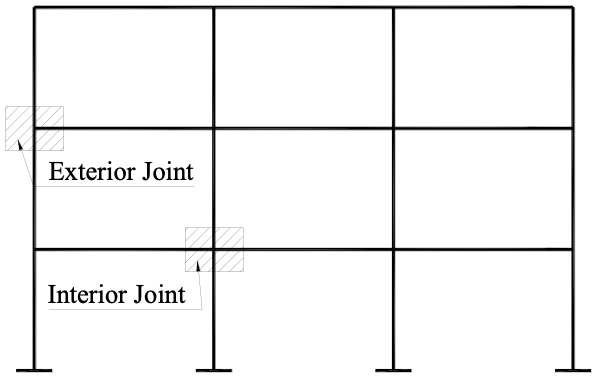
\includegraphics{images/Picture 1.png}
\caption{Exemplu de figură (sursa: Buletinul ştiinţific al UPT seria construcţii-arhitectură nr.2 /2010)}
\label{fig:fig2.1}
\end{figure}

\section{Tabele}

Tabele – tabelele se numerotează în ordinea apariției în lucrare. Alternativ, tabelele pot fi numerotate în ordine în fiecare capitol, integrând în numerotare și numărul capitolului. Fiecare tabel are număr și titlu, care se menționează deasupra tabelului, aliniat centrat. Dacă este cazul, sursa datelor se precizează între paranteze după titlul tabelului.

Toate tabelele prezentate în lucrare trebuie să fie referite în textul lucrării, trebuie să fie numerotate şi însoţite de un titlu (vezi exemplul de mai jos). Dacă se utilizează figuri copiate atunci se va indica sursa fotografiei în paranteză. Pe cât posibil, în tabel se va păstra fontul uzual (arial 12 pt) dar sunt acceptate şi modalităţi de a scoate în evidenţă rezultatele importante (bold, italic etc.)

Se va lăsa câte o linie liberă (arial 12 pt) între text şi tabel. Tabelele vor fi centrate pe pagină.

\begin{table}[ht]
\centering
\caption{Exemplu de tabel}
\label{table:table1}
\begin{tabular}{ |p{2.9cm}|p{2.45cm}|p{4cm}|p{2.45cm}|p{4cm}|  }
 \hline
  &  \multicolumn{2}{|c|}{Yield stress, fy [N/mm2]} & \multicolumn{2}{|c|}{Tensile strength, fu [N/mm2]} \\
 \hline
 Element & Mill certificate & Coupon tests & Mill certificate & Coupon tests \\
 \hline
 Beam IPE360 & 285.0 & 329.8 flange 348.4 web & 427.0 & 463.2 flange 464.0 web \\
 \hline
 Column HEB300 & 311.3 & 313.0 flange 341.8 web	& 446.0	& 449.8 flange 464.4 web \\
 \hline
 End plate & 281.0 & 248.3 & 424.7 & 416.0 \\
 \hline
 Cover plate & 296.0 & 273.2 & 443.0 & 436.7 \\
 \hline
\end{tabular}
\end{table}

\section{Formule}

Formulele utilizate în text se vor numerota în ordinea apariției în lucrare. Alternativ, formulele pot fi numerotate în ordine în fiecare capitol, integrând în numerotare și numărul capitolului. Numerotarea formulelor se face în paranteze rotunde. Se va lăsa câte o linie liberă (arial 12 pt) între text şi formulă. Formulele vor fi aliniate la dreapta.

\begin{equation}
A=\pi*r^2
\end{equation}

\section{Cod}

\begin{listing}[H]
	\begin{minted}{java}
public class Client {
    public static void main(String[] args) {
        Animal tiger = new Tiger();
        Animal parrot = new Parrot();
        tiger.breed(parrot);
    }
}
	\end{minted}
	\caption{Exemplu polimorfism de subtip - Cod client \label{cod:cod2.1}}
\end{listing}

Flexibilitatea pe care o oferă polimorfismul se poate observa în \cref{cod:cod2.1} la liniile \textit{(3)}, respectiv \textit{(4)}. Variabilele referință \textit{tiger} și \textit{parrot}, deși sunt de tip \textit{Animal}, pot referi obiecte de tipul \textit{Tiger}, respectiv \textit{Parrot}. Totuși, această flexibilitate devine o problemă în contextul apelului metodei de la linia \textit{(5)}, întrucât „împerecherea” ar avea sens doar între obiecte ale aceluiași tip.